\documentclass[11pt]{article}
\usepackage{latexsym}
\usepackage{amsmath}
\usepackage{amssymb}
\usepackage{amsthm}
\usepackage{epsfig}
\usepackage[tight]{subfigure}
\usepackage{xcolor}

\usepackage{amsmath}

\DeclareMathOperator*{\minimize}{min}
\DeclareMathOperator*{\maximize}{max}

\usepackage{algorithm}
 %on linux you may need to run sudo apt-get install texlive-full to install algorithm.sys
\usepackage{algorithmic}

\usepackage{verbatim}

\newcommand{\handout}[5]{
  \noindent
  \begin{center}
  \framebox{
    \vbox{
      \hbox to 5.78in { {#1} \hfill #2 }
      \vspace{4mm}
      \hbox to 5.78in { {\Large \hfill #5  \hfill} }
      \vspace{2mm}
      \hbox to 5.78in { {\em #3 \hfill #4} }
    }
  }
  \end{center}
  \vspace*{4mm}
}

\newcommand{\lecture}[5]{\handout{#1}{#2}{#3}{#4}{#5}}
\newcommand{\collision}[0]{\mathrm{collision}}
\newcommand{\nocollision}[0]{\overline{\collision}}

\newcommand*{\QED}{\hfill\ensuremath{\square}}

\newtheorem{theorem}{Theorem}
\newtheorem{corollary}[theorem]{Corollary}
\newtheorem{lemma}[theorem]{Lemma}
\newtheorem{observation}[theorem]{Observation}
\newtheorem{proposition}[theorem]{Proposition}
\newtheorem{definition}[theorem]{Definition}
\newtheorem{claim}[theorem]{Claim}
\newtheorem{fact}[theorem]{Fact}
\newtheorem{assumption}[theorem]{Assumption}
\newtheorem{note}[theorem]{Note}

% 1-inch margins, from fullpage.sty by H.Partl, Version 2, Dec. 15, 1988.
\topmargin 0pt
\advance \topmargin by -\headheight
\advance \topmargin by -\headsep
\textheight 8.9in
\oddsidemargin 0pt
\evensidemargin \oddsidemargin
\marginparwidth 0.5in
\textwidth 6.5in

\parindent 0in
\parskip 1.5ex
%\renewcommand{\baselinestretch}{1.25}

\begin{document}

\lecture{Statistical Techniques in Robotics (16-831, S21)}{Lecture \#10
  (Monday, March 8)}{Lecturer: Kris Kitani}{Scribes: Xuhua Huang, Xinjie Yao}{Online Techniques for Supervised Learning}

\section{Review}
In last two lectures, we start to focus on the Online Convex Optimization problem. We will give a brief recap for 3 representative algorithms (OMD, OGD, ONEGD) in this section. Then we will move on to Online Supervised Learning, and introduce two online techniques (Hard-SVM and Soft-SVM) to solve Supervised Learning problem in the online schema.

%Length requirement 1-2 pages.
        
\subsection{Online Mirror Descent (OMD)}
Online Mirror Descent (OMD) is a special instance of Follow the Regularized Leader (FTRL) by applying linear loss and convex regularizer on FTRL. It can also be viewed as a generic form of FTRL with linear loss, by changing some notations and introducing the concept of dual space and primal space:
\begin{itemize}
    \item $\boldsymbol{z}^{(1: t)}=\sum_{i=1}^{t} \boldsymbol{z}^{(i)}$ (sum of gradients)
    \item $\boldsymbol{\theta}^{(t+1)} \triangleq-\boldsymbol{z}^{(1: t)}$ (denote $\boldsymbol{\theta}$ as the sum of gradients)
    \item $\boldsymbol{\theta}^{(t+1)}=\boldsymbol{\theta}^{(t)}-\boldsymbol{z}^{(t)}$ (denote $\boldsymbol{\theta}$ as a incremental update from last timestep)
    \item $\boldsymbol{w}^{t+1} = g\left(\boldsymbol{\theta}^{(t+1)}\right) \triangleq \underset{\boldsymbol{w}}{\arg \max }\left\langle\boldsymbol{w}, \boldsymbol{\theta}^{(t+1)}\right\rangle-\psi(\boldsymbol{w})$ (mirror function from dual to primal space)
\end{itemize}
With this new notation, we can now write down the pseudo-code of OMD in Algorithm \ref{algo:OMD}.
\begin{algorithm}[H]
\caption{Online Mirror Descent (Convex set $\left.S, g: \mathbb{R}^{D} \rightarrow S\right)$}
\label{algo:OMD}
\begin{algorithmic}[1]
\FOR{$t=1,\;\cdots,\;T$}
\STATE \textsc{Receive} ($\textbf{f}^{(t)}: S\rightarrow R$) \hfill $\triangleright$ Receive loss function
\STATE  $\boldsymbol{\theta}^{(t+1)}=\boldsymbol{\theta}^{(t)}-\eta \boldsymbol{z}^{(t)}, \boldsymbol{z} \in \partial f^{(t)}\left(\boldsymbol{w}^{(t)}\right)$\hfill $\triangleright$ Dual parameter update
\STATE  $\boldsymbol{w}^{(t+1)} \leftarrow g\left(\boldsymbol{\theta}^{(t+1)}\right)$ \hfill $\triangleright$ Mirror projection
\ENDFOR
\end{algorithmic}
\end{algorithm}
OMD is an algorithm trying to solve optimization in dual space, and mirror the output back to primal space. The choice of different regularization functions can lead to different dual spaces. 

With the help of Convex Conjugate function and Bregman Divergence, we can derive the general regret bound of OMD as:
\begin{equation}
\begin{aligned}
R(\boldsymbol{u}) &=\sum_{t=1}^{T} \boldsymbol{w}^{(t)} \cdot \boldsymbol{z}^{(t)}-\boldsymbol{u} \cdot \boldsymbol{z}^{(t)} 
& \leq \psi(\boldsymbol{u})-\psi\left(\boldsymbol{w}^{(1)}\right)+\sum_{t=1}^{T} D_{\psi^{*}}\left(-\boldsymbol{z}^{(1: t)} \|-\boldsymbol{z}^{(1: t-1)}\right)
\end{aligned}
\label{eq:regretOMD}
\end{equation}
$\psi$ is the convex regularization function, and $D_{\psi^{*}}$ is the Bregman Divergence when taking the convex conjugate of the regularizer. From Equation \ref{eq:regretOMD}, we notice that choosing a different regularization function $\psi$ changes the regret bound and leads to a different algorithm.


\subsection{Online Gradient Descent (OGD)}
Gradient descent is a standard approach for minimizing differentiable convex functions. Three perspectives are introduced to understand the rationality behind.

\underline{Geometric:} An intuitive way of finding the minima of f is to move in the direction opposite of the gradient. Given a convex and differentiable function, we could approach the minima using Algorithm \ref{algo:gd}. 
\begin{algorithm}[H]
\caption{Gradient Descent ($f$)}
\label{algo:gd}
\begin{algorithmic}[1]
\STATE $\mathbf{w}^{(0)} \leftarrow \boldsymbol{0}$
\FOR{$t=1,\;\cdots,\;T$}
\STATE \textsc{Compute}($\nabla f(\mathbf{w}^{(t-1)})$)
\STATE $\mathbf{w}^{(t)} = \mathbf{w}^{(t-1)} - \eta \nabla f(\mathbf{w}^{(t-1)})$
\ENDFOR
\end{algorithmic}
\end{algorithm}
\underline{Linear approximation with regularization:} A more rigorous way is to bound this convex function f by its Taylor series approximation at $\mathbf{w}$. 

\begin{equation*}
f(\mathbf{u}) \geq f(\mathbf{w}) + \langle \mathbf{u}-\mathbf{w}, \nabla f(\mathbf{w}) \rangle
\end{equation*}
However, minimizing the RHS directly yields a solution close to negative infinity. Because Taylor series expansion is only accurate around $\mathbf{w}$, an additional constraint is included that minimizes the distance between $\mathbf{u}$ and $\mathbf{w}$ with the squared L2 norm, i.e. $\min_{\mathbf{w}}\| \mathbf{u} - \mathbf{w} \|_2^2$.  Then, the objective function becomes a linear loss with quadratic regularization.
\begin{equation*}
\mathbf{w}^{(t+1)} = 
\underset{\mathbf{w}}{\arg\min} \frac{1}{2} \| \mathbf{w} - \mathbf{w}^{(t)} \|^2 
+ \eta\Big(f(\mathbf{w}^{(t)}) + \langle \mathbf{w}-\mathbf{w}^{(t)}, \nabla f(\mathbf{w}^{(t)}) \rangle \Big)
\end{equation*}

\underline{Isometric quadratic approximation:} 
By isometric quadratic approximation, we can further derive its lower bound as 
\begin{equation*}
\begin{split}
f(\mathbf{u}) \approx f(\mathbf{w}) + (\mathbf{u}-\mathbf{w})^T \nabla f(\mathbf{w}) + \frac{1}{2\eta} (\mathbf{u}-\mathbf{w})^T \boldsymbol{I} (\mathbf{u}-\mathbf{w}),
\end{split}
\end{equation*}
It turns out to be the same objective function as the second perspective's. Then we simply use $\mathbf{w}^{(t)} = \mathbf{w}^{(t-1)} - \eta \nabla f(\mathbf{w}^{(t-1)})$ to locate its minima, which is based on a \textbf{quadratic approximation} of the loss function $f$. 
Next, we show the regret bound of online gradient descent is 
\begin{align*}
    R_{OGD} \leq DG\sqrt{T} \nonumber
\end{align*} where
\begin{align*}
    D = &\max ||\mathbf{u}||_2 \quad \mathbf{u}\in S \nonumber\\
    G = &\max ||\mathbf{z}||_2 \quad \mathbf{z}\in \partial f(\mathbf{w}) \nonumber
\end{align*}

\subsection{Online Normalized Exponentiated Gradient Descent (ONEGD)}
We have already known different regularizers can lead to different algorithms. If we stick to linear loss function, but define regularization function as: 
\begin{equation}
\psi(\boldsymbol{w})=\sum_{k=1}^{K} w_{k} \log w_{k} \quad \boldsymbol{w} \in \mathbb{S}^{K}
\end{equation}
We can have a new update rule as:
\begin{equation}
\begin{aligned}
\boldsymbol{w}^{(1+t)} 
&=\underset{\boldsymbol{w}}{\arg \min }\left\langle\boldsymbol{w},-\boldsymbol{\theta}^{(t+1)}\right\rangle+\sum_{k=1}^{K} w_{k} \log w_{k}+\lambda\left(1-\sum_{k} w_{k}\right)
\end{aligned}
\end{equation}
The extra item at the end is because using entropy regularization requires the weights sum to 1.
To solve for the minimizer, we just need to take derivative of following equation:
\begin{equation}
\mathcal{L}=\left\langle\boldsymbol{w},-\boldsymbol{\theta}^{(t+1)}\right\rangle+\frac{1}{\eta} \sum_{k=1}^{K} w_{k} \log w_{k}+\lambda\left(1-\sum_{k} w_{k}\right)
\end{equation}
and get the minimizer:
\begin{equation}
w_{n}=\frac{\exp \left(\eta \theta_{k}\right)}{\exp (1-\eta \lambda)}
\end{equation}
which can be viewed as a mirror projection from dual space to primal space.
\begin{algorithm}[H]
\caption{ Online Norm-Exp-GD ($\eta$)}
\label{algo:onegd}
\begin{algorithmic}[1]
\FOR{$t=1,\;\cdots,\;T$} %
\STATE $\boldsymbol{\theta}^{(t+1)}=\boldsymbol{\theta}^{(t)}-\eta \boldsymbol{z}^{(t)}, \quad \boldsymbol{z}^{(t)} \in \partial f^{(t)}\left(\boldsymbol{w}^{(t)}\right)$ \hfill $\triangleright$ Dual parameter update
\STATE $\boldsymbol{w}^{(t+1)} \propto \exp \left(\eta \boldsymbol{\theta}^{(t+1)}\right)$ \hfill $\triangleright$ Mirror projection
\ENDFOR
\end{algorithmic}
\end{algorithm}


\section{Summary}
Before we dive into the algorithms for Online Supervised Learning, it is better to connect it with Online Learning and Supervised Learning by Figure \ref{fig:OLSL}. Though some supervised learning problems will perform a batch learning and only test after training the algorithm offline, there are still some scenarios where online techniques would be more suitable. For example, there are tons of Go playing strategies for AlphaGo to learn from, it is not reasonable to test its performance and update parameters after going through all data. Therefore, we may introduce the Online Learning schema (training + testing loop) into Supervised Learning, which is Online Supervised Learning we are going to discuss.

\begin{figure}[H]
\centering
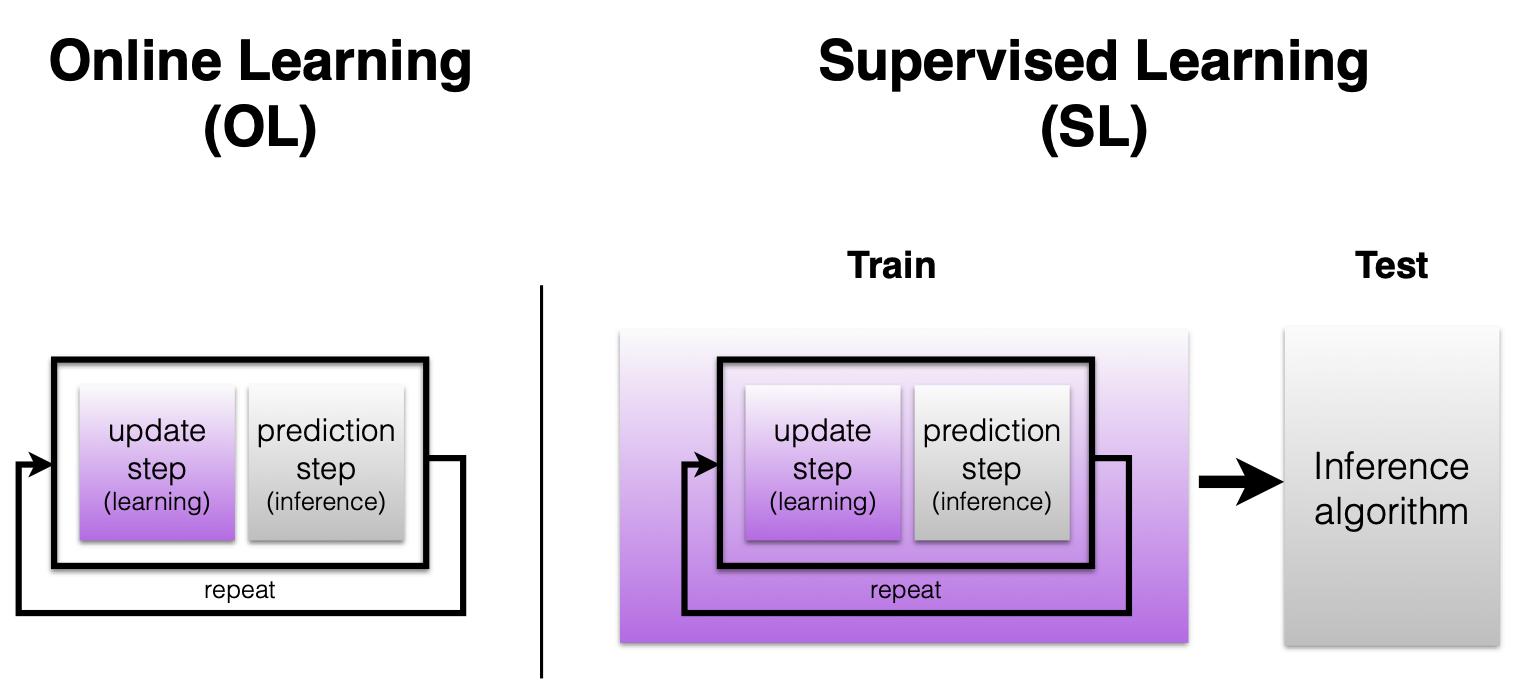
\includegraphics[width=0.8\textwidth]{OLSL.png}
\caption{Online Learning vs. (Online) Supervised Learning}
\label{fig:OLSL}
\end{figure}

\subsection{Hyperplane}
First we need to review some fundamental concepts about Hyperplane.
\subsubsection{Hyperplane in 2D}
As shown in Figure \ref{fig:hyperplane}, in 2D, hyperplane is a line denoted as $\mathbf{w}\cdot\mathbf{x} + b = 0$, where $\mathbf{w}$ and $\mathbf{x}$ are $2\times1$ vector. We can also notice that scaling $\mathbf{w}$ by any factor will still give a same hyperplane. 
\lemma{The distance from a point to a line can be written as:
\begin{equation}
\operatorname{distance}\left(w_1 x+w_2y+b=0,\left(x_{0}, y_{0}\right)\right)=\frac{\left|w_1 x_{0}+w_2 y_{0}+b\right|}{\sqrt{w_1^{2}+w_2^{2}}}
\end{equation}}
\normalfont
Therefore, by plugging in the origin point $(0,0)$, we can have distance $\rho=\frac{b}{\|\boldsymbol{w}\|}$. When we have two hyperplane $\mathbf{w}\cdot\mathbf{x} + b = 0$ and $\mathbf{w}\cdot\mathbf{x} + b = -1$, their difference of distance from origin will be:
\begin{equation}
\frac{b+1}{\|\boldsymbol{w}\|}-\frac{b}{\|\boldsymbol{w}\|}=\frac{1}{\|\boldsymbol{w}\|}
\end{equation}

\begin{figure}[H]
\centering
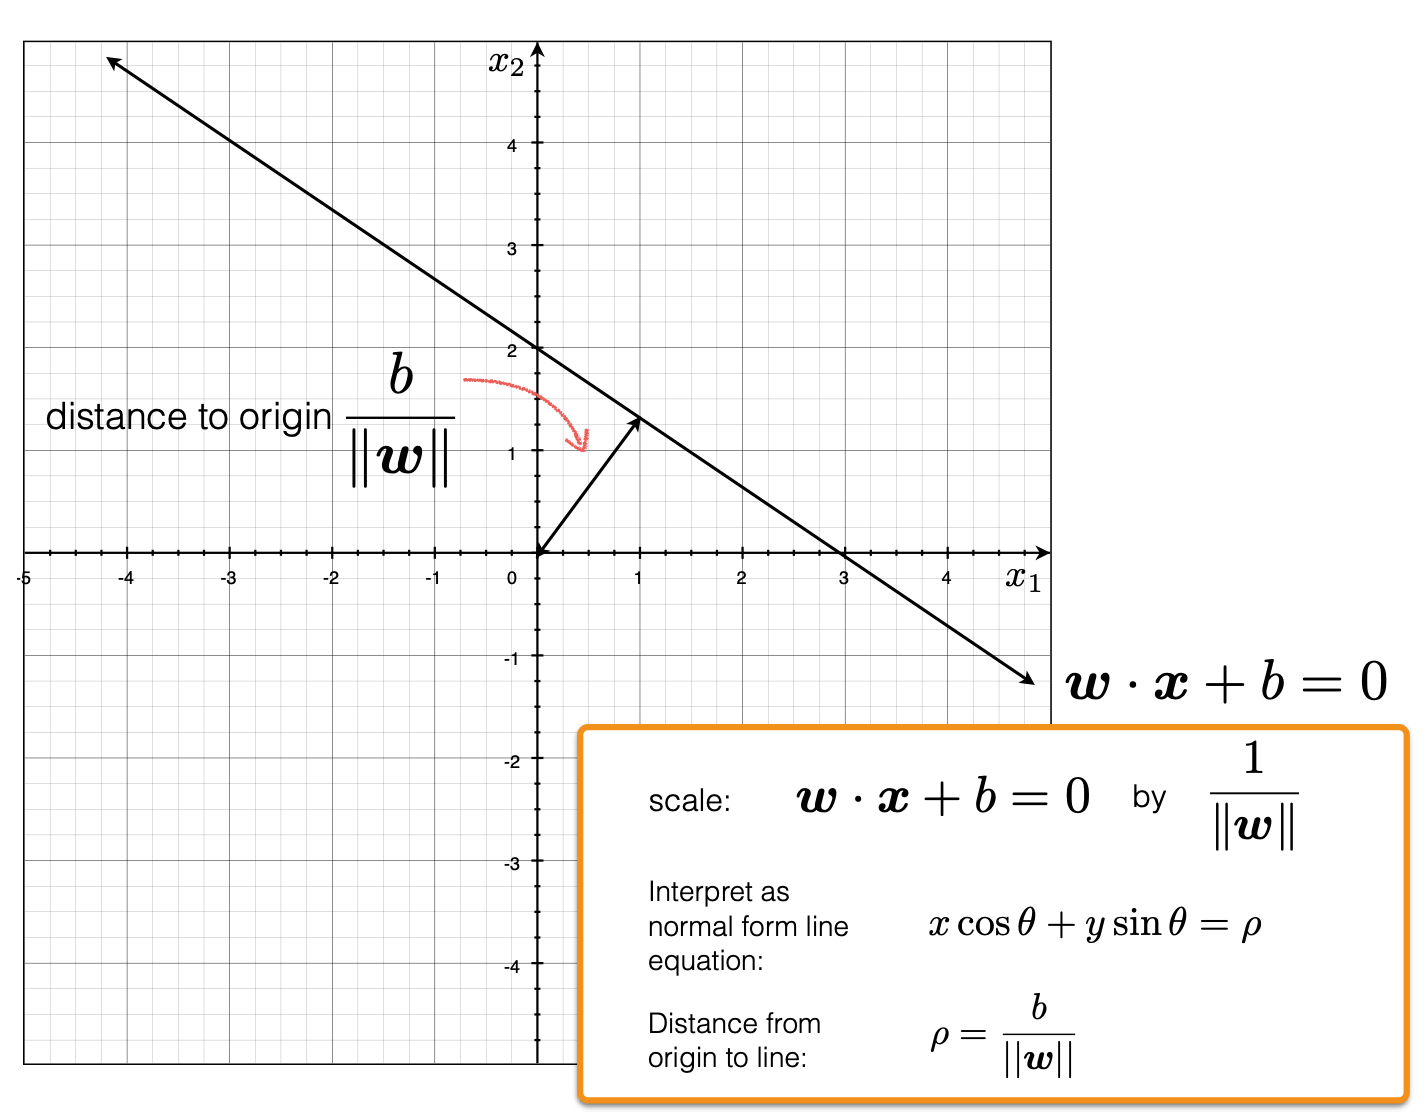
\includegraphics[width=0.5\textwidth]{hyperplane.png}
\caption{Illustration of Hyperplane in 2D and its distance from origin}
\label{fig:hyperplane}
\end{figure}

\subsubsection{Hyperplane in 3D}
The distance formula still holds in 3D coordinate. The distance indicated by the blue arrow in Figure \ref{fig:3dhyper} can be derived by:
\begin{equation}
\frac{b+1}{\|\boldsymbol{w}\|}-\frac{b-1}{\|\boldsymbol{w}\|}=\frac{2}{\|\boldsymbol{w}\|}
\end{equation}

\begin{figure}[H]
\centering
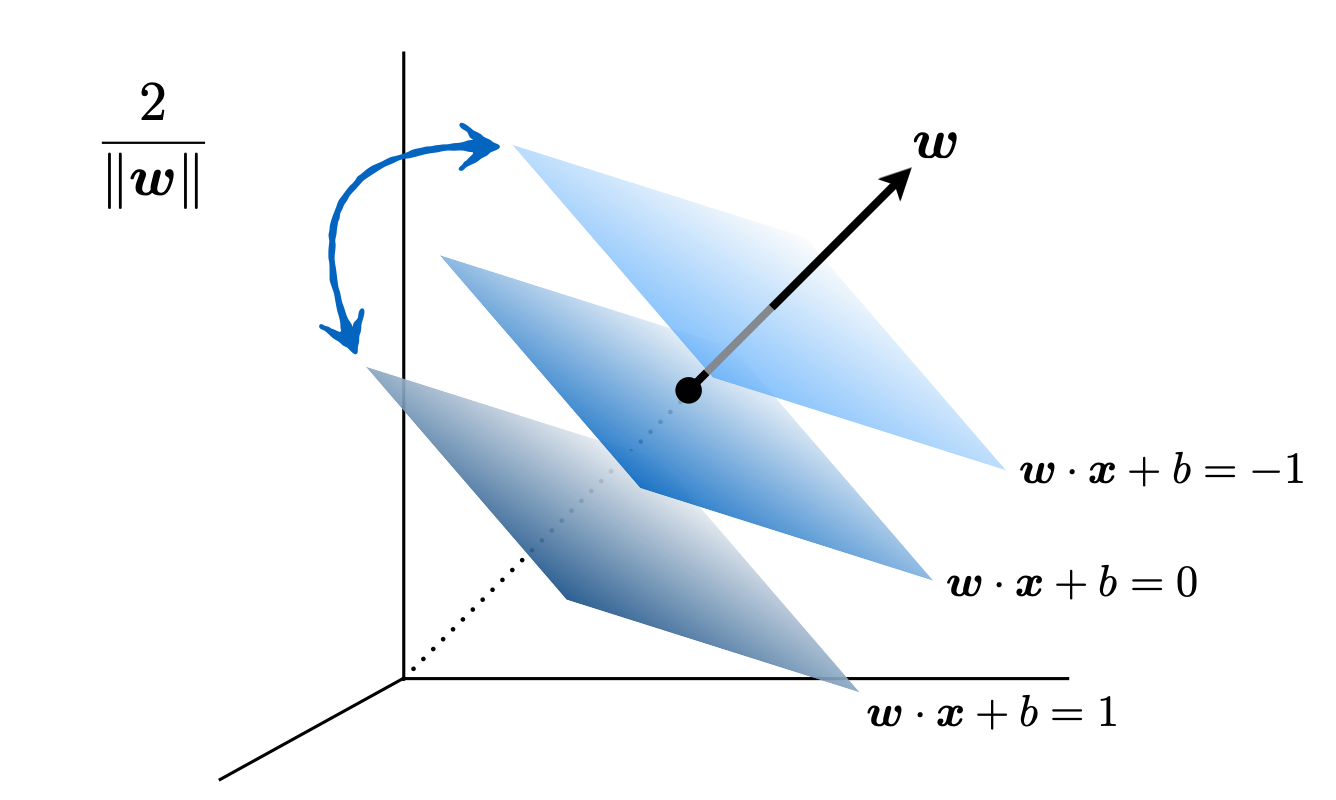
\includegraphics[width=0.5\textwidth]{3d_hyperplane.png}
\caption{Illustration of Hyperplane in 3D and distance between two hyperplanes}
\label{fig:3dhyper}
\end{figure}


\subsection{Support Vector Machine (SVM)}

\subsubsection{Margin}
\label{sec:margin}
\definition{Margin is the distance from the decision hyperplane to the closest data point (on both sides).}

\normalfont
The best hyperplane should be maximally far away from any data point. As visualized in Figure \ref{fig:margin}, to find an optimal $\mathbf{w}$, we must find a hyperplane which can maximize the distance between two parallel hyperplanes (i.e. $\frac{2}{\|\mathbf{w}\|}$).


\begin{figure}[H]
\centering
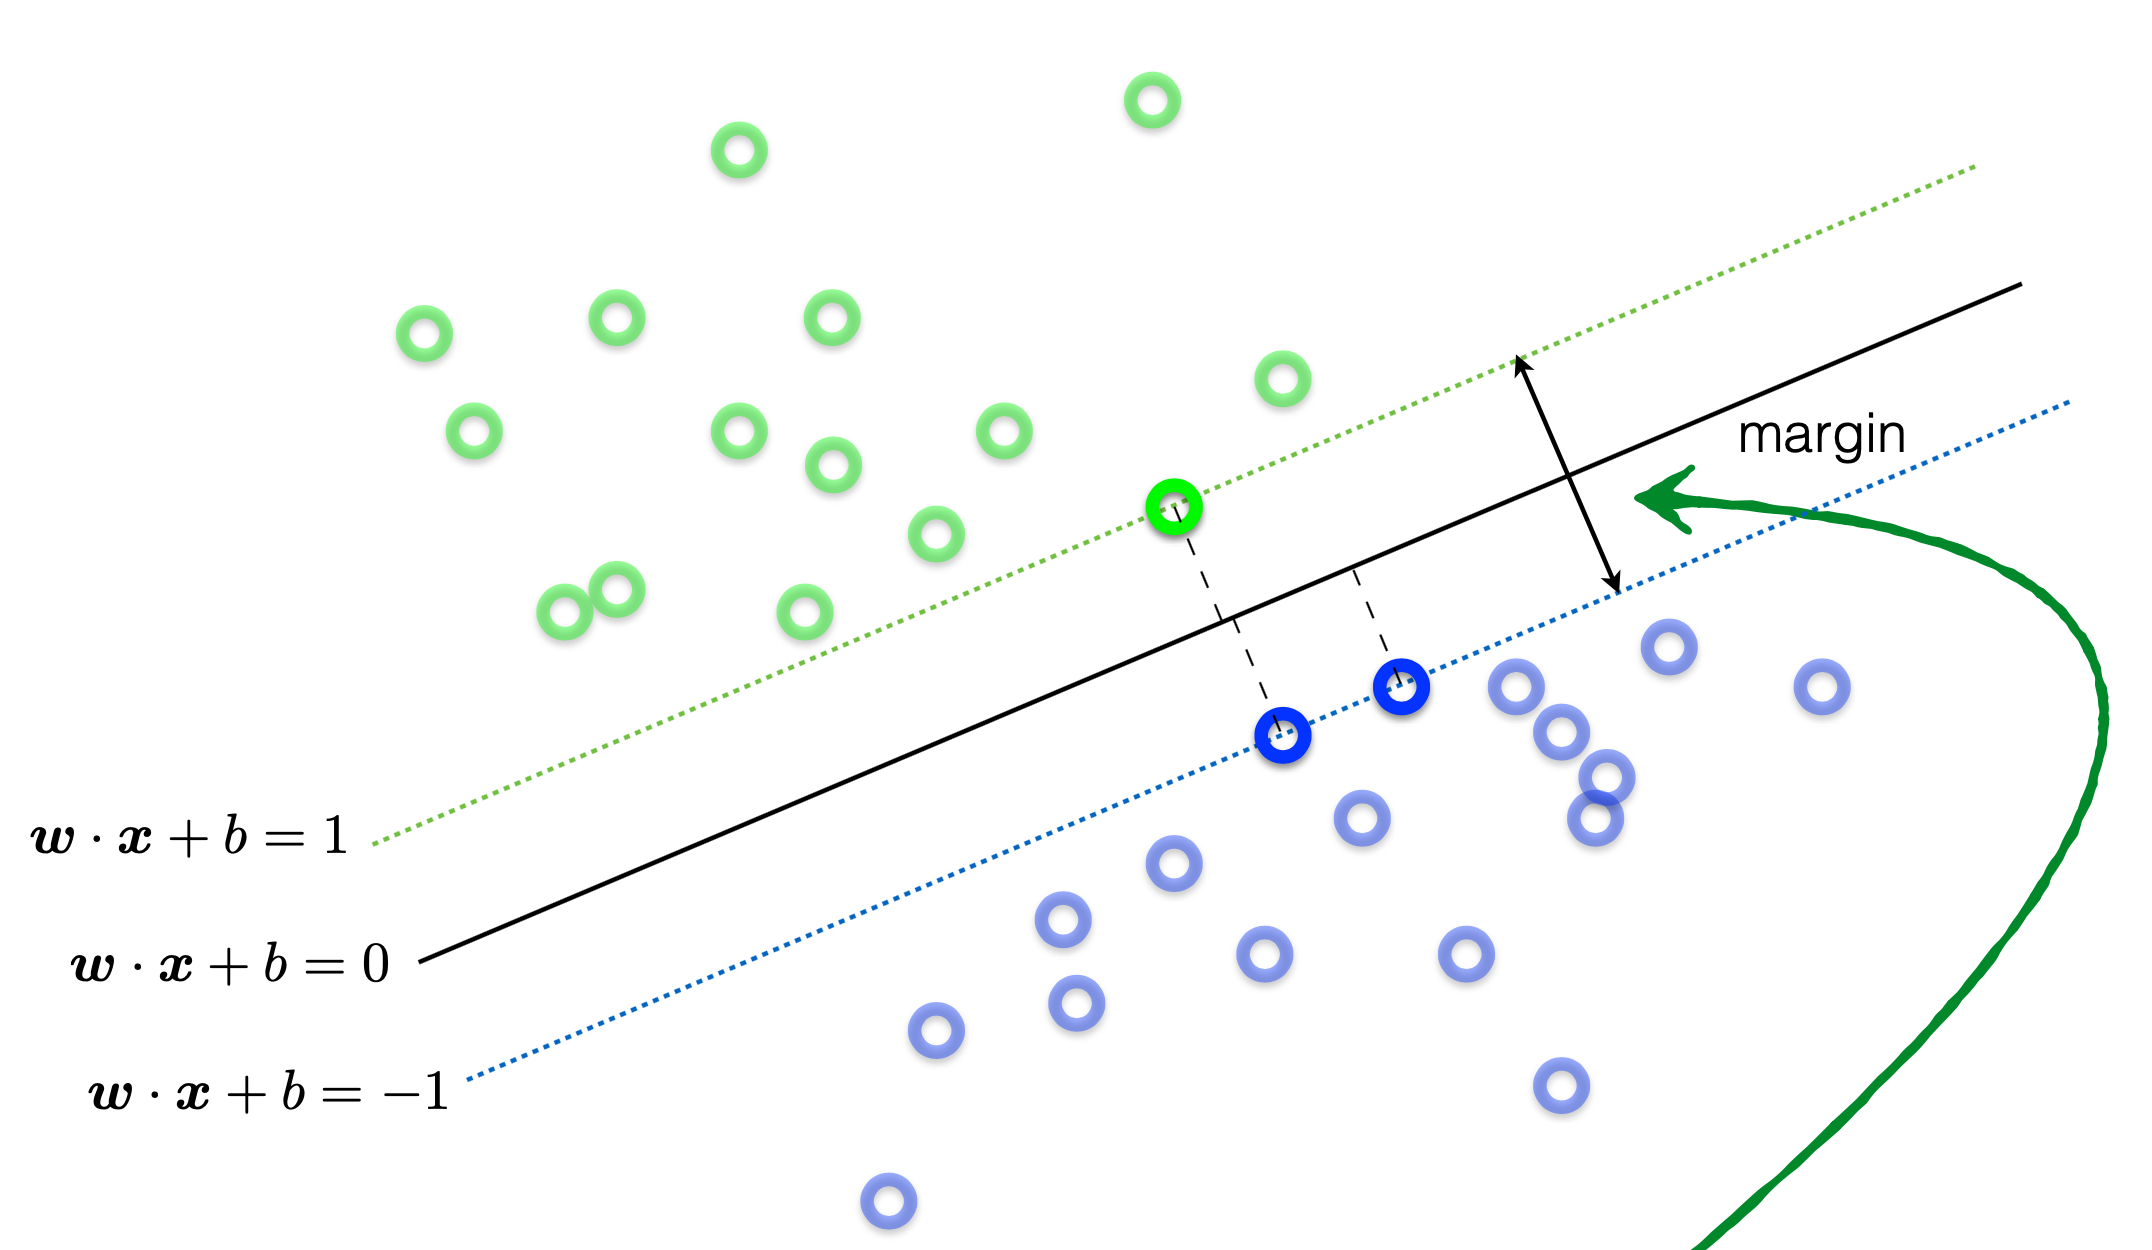
\includegraphics[width=0.5\textwidth]{margin.png}
\caption{Illustration of optimal margin}
\label{fig:margin}
\end{figure}

\subsubsection{Hard Margin SVM}
Based on the definition in Section \ref{sec:margin}, we can now define Linear SVM as a algorithm to find a hyperplane maximizing the margin:
\begin{equation}
\begin{array}{c}
\max\limits_{\boldsymbol{w}} \frac{2}{\|\boldsymbol{w}\|} \\
\text { subject to } \boldsymbol{w} \cdot \boldsymbol{x}_{i}+b \begin{array}{l}
\geq+1 \text { if } y_{i}=+1 \\
\leq-1 \text { if } y_{i}=-1
\end{array} \text { for } i=1, \ldots, N
\end{array}
\label{eq:svm1}
\end{equation}
To make it as a convex quadratic programming (QP) problem, we can convert the objective function as:
\begin{equation}
\begin{array}{c}
\min _{\boldsymbol{w}}\|\boldsymbol{w}\|^{2} \\
\text{ subject to } y_{i}\left(\boldsymbol{w} \cdot \boldsymbol{x}_{i}+b\right) \geq 1 \text{ for } i=1, \ldots, N
\end{array}
\label{eq:hardsvm}
\end{equation}
where $y_{i}\left(\boldsymbol{w} \cdot \boldsymbol{x}_{i}+b\right) \geq 1$ is just a restatement of constraint in Equation \ref{eq:svm1}.
\note{Equation \ref{eq:hardsvm} is a maximization problem with \textit{hard} constraints, by enforcing correct classification of all points.}

\normalfont
\subsection{Soft Margin SVM}
In real world setting, the training data can be noisy or even non-separable, which makes it impossible to find a hyperplane perfectly classifies the data. Therefore, we should allow certain degree of mistakes in order to avoid overfitting and to make our decision hyperplane more robust. This leads to the soft margin version of SVM, by adding a positive slack variable $\xi_{i}$ in the criterion: 
\begin{equation}
y_{i}\left(\boldsymbol{w}^{\top} \boldsymbol{x}_{i}+b\right) \geq 1-\xi_{i}
\end{equation}
We can treat $\xi_{i}$ as the distance from the misclassified point to its corresponding margin. Intuitively, if its value becomes larger, it will allow more mistakes and the constraint will become softer.

With this new constraint, we can change our objective to:
\begin{equation}
\begin{array}{c}
\min\limits_{\boldsymbol{w}, \boldsymbol{\xi}}\|\boldsymbol{w}\|^{2}+C \sum_{i} \xi_{i} \\
\text{ subject to } y_{i}\left(\boldsymbol{w}^{\top} \boldsymbol{x}_{i}+b\right) \geq 1-\xi_{i}
\text{ for }i=1, \ldots, N
\end{array}
\end{equation}
where we allow a slack variable in the constraint but still want to keep it as small as possible. $C$ is a regularization hyperparameter, if we apply a small $C$, it will ignore the value of $\xi$, which basically allows mislabeling every data label, and generate a larger margin (soft margin). On the contrary, with a large $C$, we emphasize more on constraints and make the margin smaller (hard margin). 

One way to formulate the objective function is as,
\begin{align}
\min_\mathbf{w} \left(\frac{\lambda}{2}||\mathbf{w}||^2 + \frac{1}{M} \sum_{m=1}^{M} (1 - y_m\mathbf{w}^T\mathbf{x}_m) \right)
\end{align}
However, the slack value $(1 - y_m\mathbf{w}^T\mathbf{x}_m)$ does not perform as what we want. It causes correct points with large negative values over-weigh the misclassified points with small values. Instead, it is supposed to penalize for misclassified points or weakly correct points (ignoring the very correct points). 
By replacing the slack value with a hinge loss, we achieve a convex and non-differentiable optimization function.
\begin{align}
\min_\mathbf{w} \left(\frac{\lambda}{2}||\mathbf{w}||^2 + \frac{1}{M} \sum_{m=1}^{M} \max \{0,1 - y_m\mathbf{w}^T\mathbf{x}_m\} \right)
\end{align}

\subsubsection{Online sub-gradient descent} 
\lemma{Gradient descent requires a convex and differentiable loss function.\label{lemma:diffloss}}

\definition{A \textbf{sub-gradient} is any $g \in \Re^n$ (same dimension as $x$) such that:
\[
f(y) \geq f(x) + g^T (y - x), \>\> \forall y
\]}
\definition{Set of sub-gradients at $x=w$ is the \textbf{differential set} for $f(w)$.}

\normalfont
As the loss function is convex but non-differentiable, we will apply sub-gradient descent to find the minima according to lemma \ref{lemma:diffloss}. Online sub-gradient descent uses any one from the set of sub-gradients at the non-differentiable points.

\normalfont
We consider two possible cases for sub-gradients of the hinge loss. One is when data points are correctly classified, sub-gradient $z_m$ is set to 0. The other is when data points lie within the margin or are misclassified, sub-gradient is set to $-y_m\mathbf{x}_m$. 
\[ \mathbf{z}_m =
    \begin{cases}
         \mathbf{0} & 
         \text{if  $y_m\mathbf{w}^T\mathbf{x}_m \geq 1$,}\\
        -y_m\mathbf{x}_m & \text{otherwise}
    \end{cases}
\]
Then we can write the algorithm in online mirror descent form as Algorithm \ref{algo:SoftSVM}. 
\begin{algorithm}[H]
\caption{SoftSVM($\lambda$)}
\label{algo:SoftSVM}
\begin{algorithmic}[1]
\STATE $\boldsymbol{\theta}^{(1)} \leftarrow \mathbf{0} \in \mathbb{R}^N$
\FOR{$t=1,...,T$}
\STATE $\boldsymbol{x_d}, y_d \sim \boldsymbol{D}$ \hfill $\triangleright$ Receive sample from environment
\STATE $\boldsymbol{\theta}^{(t)} = \boldsymbol{\theta}^{(t-1)} + y_d\boldsymbol{x_d}\cdot\textbf{1}[y_d(\boldsymbol{w}^{(t)}\cdot \boldsymbol{x_d}) < 1]$ \hfill $\triangleright$ Dual parameter update
\STATE $\boldsymbol{w}^{(t+1)} \leftarrow \frac{1}{\lambda (t+1)}\boldsymbol{\theta}^{(t)}$ \hfill $\triangleright$ Mirror Projection
\ENDFOR
\STATE $\boldsymbol{\bar{w}} = \frac{1}{T}\sum_t \boldsymbol{w^{(t)}}$
\end{algorithmic}
\end{algorithm}

\subsubsection{Comparison with Perceptron}
Recall Perceptron algorithm written in online mirror descent form as Algorithm \ref{algo:perceptron_omd},
\begin{algorithm}[H]
\caption{Perceptron}
\label{algo:perceptron_omd}
\begin{algorithmic}[1]
\STATE $\boldsymbol{w}^{(1)} \leftarrow 0$ 
\FOR{t=1,...,T}
\STATE RECEIVE $(\boldsymbol{x}^{(t)}, y^{(t)}) \in \mathbb{R}^N$ \hfill $\triangleright$ Receive sample from environment
\STATE $\boldsymbol{\theta}^{(t)} = \boldsymbol{\theta}^{(t-1)} + y^{(t)}\boldsymbol{x}^{(t)}\cdot\textbf{1}[y^{(t)}\langle \boldsymbol{w}^{(t)}, \boldsymbol{x}^{(t)} \rangle  < 0]$ \hfill $\triangleright$ Dual parameter update
\STATE $\boldsymbol{w}^{(t+1)} \leftarrow \boldsymbol{\theta}^{(t)}$ \hfill $\triangleright$ Mirror Projection
\ENDFOR
\end{algorithmic}
\end{algorithm}

\observation{ There are some similarities and differences between Perceptron algorithm and SoftSVM algorithm.
\begin{enumerate}
    \item Both of them have piece-wise linear loss with quadratic regularization.
    \item Dual parameter update diverges: SoftSVM allows a soft margin while Perceptron uses no margin.
    \item Mirror function differs: SoftSVM has a multiplication update while Perceptron uses an identity mapping (step size could be applied to Perceptron).
\end{enumerate}
}

\normalfont
\subsection{Conclusion}
In this lecture, we dive into the Online Supervised Learning problem, by introducing a representative algorithm called Support Vector Machine (SVM). We turn it into an online learning algorithm by introducing the hinge loss and sub-gradient descent. To handle non-separable or noisy data, we allow it to have a soft margin, aiming to make it more robust in testing environment. SVM can be written in the form of OMD. Interestingly, it is very similar to Perceptron while they are slightly different in the dual parameter update and mirror function.
\newpage

\section{Appendix}
\subsection{More on Online SVM} 
Under the online learning setting, SVM is continuously being trained with real-time data input coming in. One of the most popular online SVM solver is called \textbf{LASVM} proposed in \cite{lasvm}. LASVM is used for big data stream mining, and was introduced by Bordes in 2005. Figure \ref{fig:lasvm} shows the overall pipeline for LASVM, please refer to the paper to get more details. The basic idea is to incorporate SVM with online kernel classifiers. The algorithm uses the traditional SVM (Quadratic Programming) solver with online kernel approximation which leverages a similar single sequential pass method used in SVM \cite{iunera_2020}.
\begin{figure}[H]
\centering
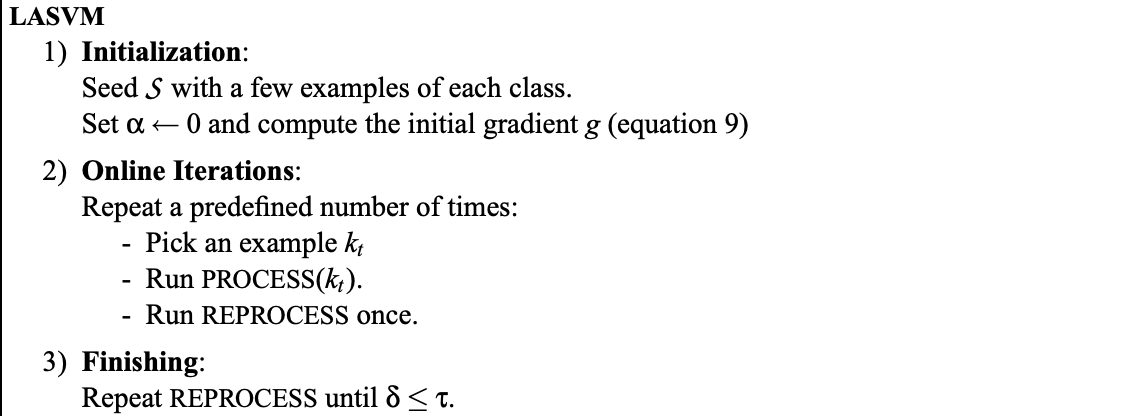
\includegraphics[width=1.0\textwidth]{LASVM.png}
\caption{LASVM algorithm}
\label{fig:lasvm}
\end{figure}

\subsection{Comparison between online SVM and offline SVM} 
There are two insightful tables for comparing online SVM and offline SVM from \cite{iunera_2020}.

In terms of the data types, constant and small data set size may be more suitable for offline SVM, whereas a continuously changing data will be most suitable to online SVM. Online SVM can handle stationary and non-stationary data where it is continuously changing its patterns.

\begin{figure}[H]
\centering
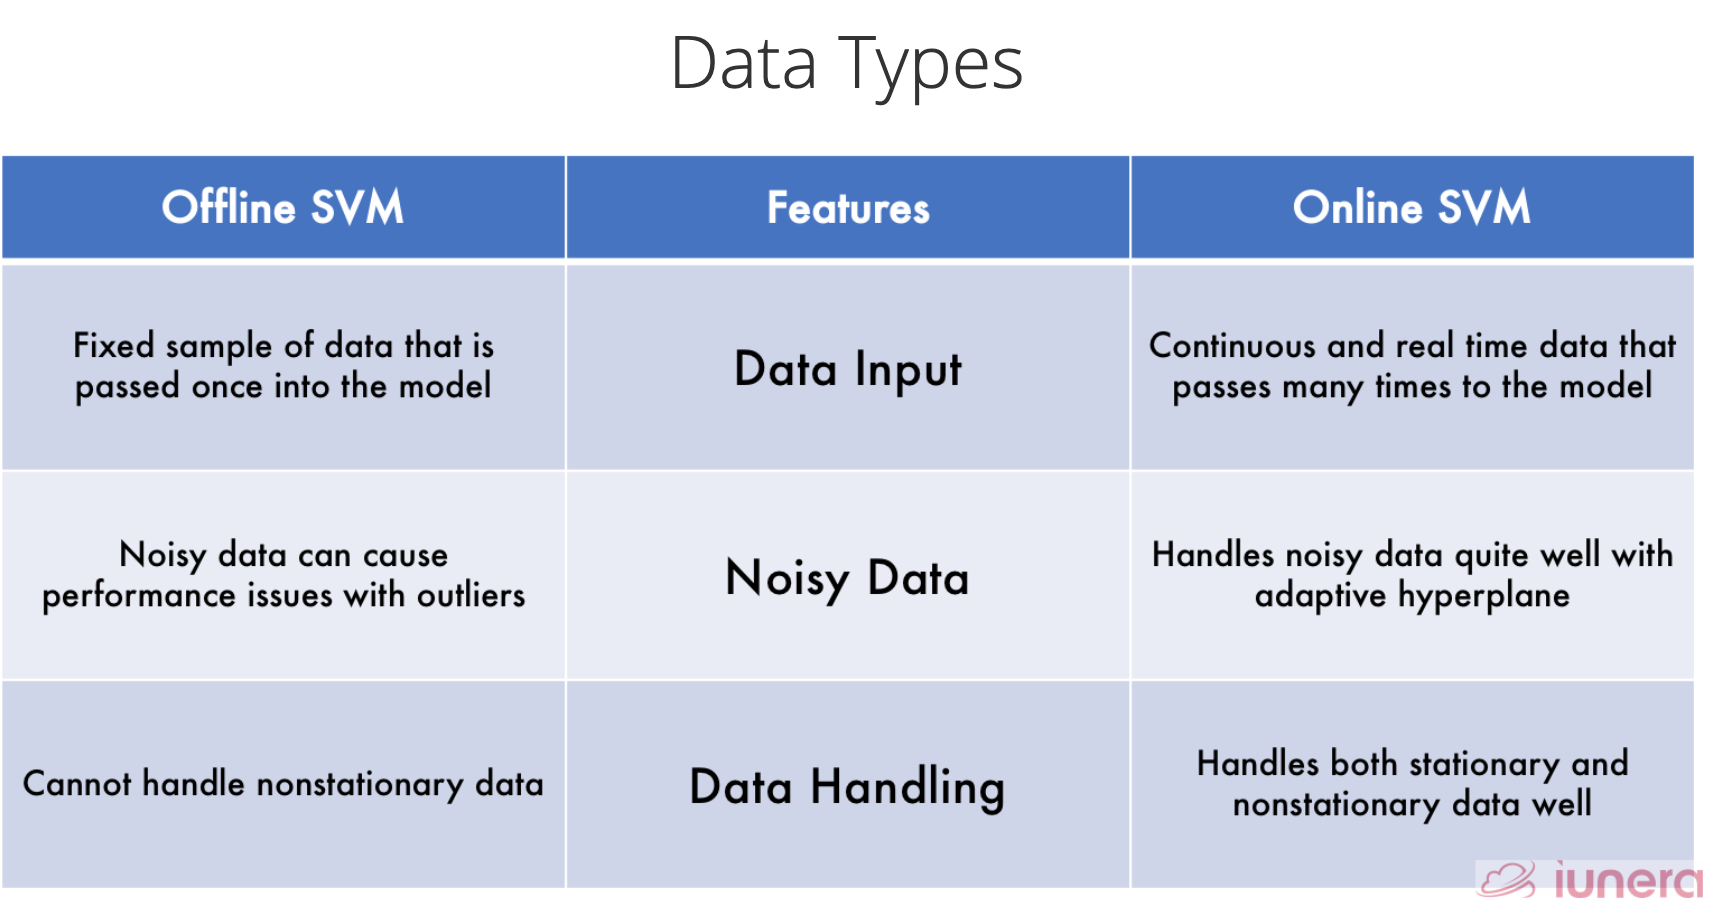
\includegraphics[width=0.7\textwidth]{com1.png}
\caption{Comparison in data types}
\label{fig:com1}
\end{figure}

In terms of model features, online SVM is less complex in handling data of different patterns due to its ability to re-train the algorithm when a new sample is given. It is able to adapt to data input stream and to adjust accordingly.

\begin{figure}[H]
\centering
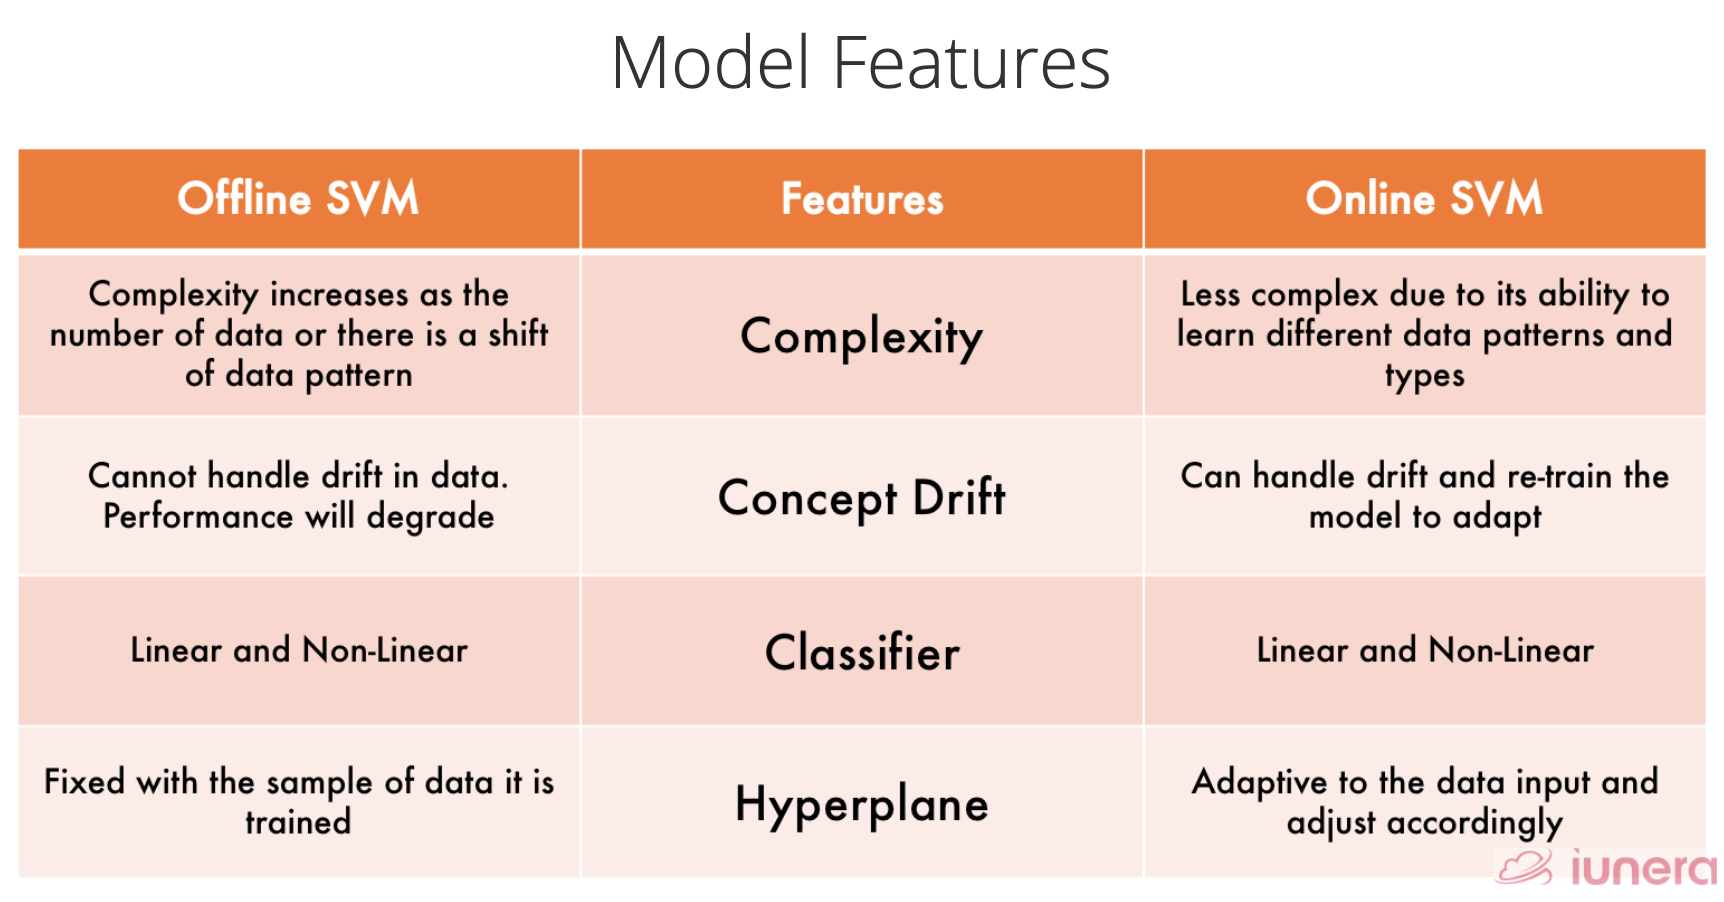
\includegraphics[width=0.7\textwidth]{com2.png}
\caption{Comparison in model features}
\label{fig:com2}
\end{figure}


\subsection{Other good matrials for SVM / Online SVM}
\begin{itemize}
    \item Introduction to Support Vector Machine: http://cs229.stanford.edu/notes/cs229-notes3.pdf
    \item Support Vector Machines for Classification: \textit{https://www.ugpti.org/smartse/resources/downloads/support-vector-machines.pdf}
    \item Linear and Non Linear Classifier: \textit{https://towardsdatascience.com/understanding-support-vector-machine-part-2-kernel-trick-mercers-theorem-e1e6848c6c4d}
    \item Active Support Vector Machine: \textit{http://sdep.cs.aueb.gr/docs/Vlachos-Active-Learning-MScThesis.pdf}
\end{itemize}



%\section*{References}
%Include your references here. Please cite any resources you found useful.	
%Populate the refs.bib file or list your references manually. Be consistent in formatting!
{
\bibliography{refs}
\bibliographystyle{abbrv}
}

%\section{Appendix}
%This section provides any relevant background material that was not covered in the lectures, but was found to be useful for understanding the material. 
%For example, derivations, theory underlying techniques employed, etc. 

%Additionally, this section can summarizes applications or extensions of these techniques found in the literature. 

\end{document} % Done!


